\documentclass[11pt,a4paper]{article}

% -- Packages ------------------------------------------------------------------
\usepackage[margin=2.5cm]{geometry}
\usepackage{amsmath,amssymb}
\usepackage{booktabs}
\usepackage{multirow}
\usepackage{array}
\usepackage{pgfplots}
\pgfplotsset{compat=1.18}
\usepackage{pgfplotstable}
\usepackage{hyperref}
\usepackage{caption}
\usepackage{subcaption}
\usepackage{authblk}
\usepackage{microtype}
\usepackage{siunitx}
\sisetup{round-mode=places, round-precision=2}

% -- Meta ----------------------------------------------------------------------
\title{\textbf{Experimental Analysis of Strip Packing Algorithms}\\[0.4em]
       \large Comparative Study of Exact, Constructive, and Shelf Heuristics\\
       with Machine Learning Algorithm Selection}
\author{Andrei Mărisac}
\affil{Facultatea de Informatică\\Universitatea Alexandru-Ioan Cuza Iași}
\affil{}
\date{May 2026}

\begin{document}
\maketitle
\tableofcontents
\bigskip

% -- Abstract ------------------------------------------------------------------
\begin{abstract}
We present an experimental analysis of seven algorithm families for the
Two-Dimensional Strip Packing Problem (2SP): the Bottom-Left-Fill (BLF)
constructive heuristic with four sorting strategies, the Next Fit Decreasing
Height (NFDH) and First Fit Decreasing Height (FFDH) shelf heuristics,
the Skyline heuristic (four sorting strategies), a Simulated Annealing (SA)
metaheuristic, and an exact method based on Google OR-Tools CP-SAT.
Experiments on 60 benchmark instances (Bengtsson 1982; Berkey \& Wang 1987;
Martello \& Vigo 1998) show that BLF achieves a mean gap of 8.1\% above the
area lower bound, while the Skyline heuristic produces significantly larger gaps
(mean 21.6\%) due to its inability to fill concave cavities below tall items.
SA, using Skyline as an inner evaluator, achieves a mean gap of 9.9\%
on random instances with a 5\,s budget, beating BLF best-of-four on 14 of 16
tested instances.
We train two ML algorithm selectors on 17 geometric features: a Random Forest
(RF) achieving 45\% exact accuracy and 0.75\% mean regret on a 100-instance
held-out test set, and a PyTorch MLP achieving 34\% accuracy with 0.94\%
mean regret.
Even on misclassified instances both models incur sub-1\% height regret,
confirming the practical value of data-driven algorithm selection.
\end{abstract}

% ------------------------------------------------------------------------------
\section{Introduction}
% ------------------------------------------------------------------------------

The \emph{Two-Dimensional Strip Packing Problem} (2SP) asks: given a strip of
fixed width \(W\) and an unbounded height, and a set of \(n\)
axis-aligned rectangles \(\{(w_i, h_i)\}_{i=1}^{n}\), pack all rectangles
into the strip without overlap and minimise the resulting height \(H\).
The problem is NP-hard in the strong sense \cite{GareyJohnson1979}.

Practical applications include paper and sheet metal cutting, VLSI floorplanning,
advertisement placement, and container loading.
This report evaluates the algorithms listed in Table~\ref{tab:algorithms}.

\begin{table}[h]
\centering
\caption{Algorithms studied in this report.}
\label{tab:algorithms}
\begin{tabular}{llll}
\toprule
\textbf{ID} & \textbf{Algorithm} & \textbf{Class} & \textbf{Complexity} \\
\midrule
BLF-DH & BLF, Decreasing Height    & Constructive heuristic & $O(n^3)$ \\
BLF-DW & BLF, Decreasing Width     & Constructive heuristic & $O(n^3)$ \\
BLF-DA & BLF, Decreasing Area      & Constructive heuristic & $O(n^3)$ \\
BLF-DP & BLF, Decreasing Perimeter & Constructive heuristic & $O(n^3)$ \\
NFDH   & Next Fit Decreasing Height  & Shelf heuristic      & $O(n\log n)$ \\
FFDH   & First Fit Decreasing Height & Shelf heuristic      & $O(n^2)$ \\
Sky-DH & Skyline, Decreasing Height  & Skyline heuristic    & $O(n^2)$ \\
Sky-DW & Skyline, Decreasing Width   & Skyline heuristic    & $O(n^2)$ \\
Sky-DA & Skyline, Decreasing Area    & Skyline heuristic    & $O(n^2)$ \\
Sky-DP & Skyline, Decreasing Perimeter & Skyline heuristic  & $O(n^2)$ \\
SA     & Simulated Annealing (Skyline inner) & Metaheuristic  & $O(n\cdot\mathit{iter})$ \\
CP-SAT & OR-Tools CP-SAT         & Exact (60\,s limit)  & Exponential \\
ML-RF  & Random Forest Selector  & Algorithm selection  & $O(1)$ inference \\
ML-MLP & Neural Network (MLP)    & Algorithm selection  & $O(1)$ inference \\
\bottomrule
\end{tabular}
\end{table}

% ------------------------------------------------------------------------------
\section{Problem Formulation}
% ------------------------------------------------------------------------------

Let \(\mathcal{R} = \{(w_i, h_i)\}_{i=1}^n\) be the set of rectangles and
\(W \in \mathbb{Z}^+\) the strip width.
The placement of rectangle \(i\) is determined by its bottom-left corner
\((x_i, y_i)\).
The optimisation problem is:
\begin{align}
\text{minimise} \quad & H \label{eq:obj}\\
\text{subject to} \quad
  & x_i + w_i \le W, \quad y_i + h_i \le H, \quad x_i,y_i \ge 0
    \quad \forall i \label{eq:bounds}\\
  & \text{no overlap between any two rectangles.} \label{eq:nooverlap}
\end{align}

A useful lower bound is the \emph{area lower bound}:
\begin{equation}
\mathrm{LB}_{\text{area}} = \left\lceil \frac{\sum_{i=1}^n w_i h_i}{W} \right\rceil.
\label{eq:lb}
\end{equation}
The \emph{gap} of a solution with height \(H\) relative to this bound is:
\begin{equation}
\mathrm{Gap} = \frac{H - \mathrm{LB}_{\text{area}}}{\mathrm{LB}_{\text{area}}} \times 100\%.
\label{eq:gap}
\end{equation}

% ------------------------------------------------------------------------------
\section{Algorithms}
% ------------------------------------------------------------------------------

\subsection{Bottom-Left-Fill (BLF)}

BLF is a greedy constructive heuristic introduced by Baker et al.~\cite{Baker1980}
and formalised by Chazelle~\cite{Chazelle1983}.
After sorting the rectangles by a chosen key, each rectangle is placed at
the \emph{lowest} feasible $y$-coordinate, then as far \emph{left} as
possible at that level.
Candidate $y$-levels are $\{0\} \cup \{y_j + h_j : j \text{ placed}\}$, i.e.\
the bottom of the strip or the top edge of any placed rectangle.
Similarly, candidate $x$-positions are $\{0\} \cup \{x_j + w_j\}$.

Four item orderings are compared:
\textbf{DH} (decreasing height), \textbf{DW} (decreasing width),
\textbf{DA} (decreasing area), and \textbf{DP} (decreasing perimeter).

\subsection{Shelf Heuristics (NFDH, FFDH)}

Shelf heuristics \cite{Coffman1980} pack items in horizontal \emph{shelves}.
Items are sorted by decreasing height.

\textbf{NFDH}: keeps one open shelf; when the next item does not fit horizontally,
closes the shelf and starts a new one.
Approximation ratio: $H \le 2 \cdot \mathrm{OPT} + h_{\max}$.

\textbf{FFDH}: for each item scans all open shelves from the bottom and
places it on the \emph{first} shelf where it fits; opens a new shelf only if
none suffices.
Approximation ratio: $H \le \tfrac{17}{10} \cdot \mathrm{OPT} + h_{\max}$.

\subsection{Skyline Heuristic}

The \emph{Skyline} heuristic \cite{Burke2004} maintains a step-function
profile of the packing surface — the ``skyline'' — as a list of left-edge
events $(x_i, h_i)$ sorted by $x_i$.
Each event records the top height starting at $x_i$; the last segment
implicitly extends to $W$.
The initial skyline is $\{(0,0)\}$ (an empty strip).

Placing a rectangle of size $w \times h$:
\begin{enumerate}
  \item For each segment start $x_i$ with $x_i + w \le W$, compute
        $y = \max_{j:\, x_i \le x_j < x_i+w} h_j$ (highest point in
        the span $[x_i, x_i{+}w)$).
  \item Choose $x^* = \arg\min_{x_i}(y + h)$ (lowest resulting top edge).
  \item Place at $(x^*, y)$ and update the skyline: insert new events,
        clip existing ones, and merge adjacent segments of equal height.
\end{enumerate}
Rectangles are sorted by one of the four strategies (DH, DW, DA, DP).
Time complexity is $O(n^2)$: each of the $n$ placements scans at most $n$
skyline segments; sorting adds $O(n \log n)$.

\paragraph{Limitation.}
The Skyline tracks only the \emph{topmost} surface and cannot fill
\emph{caves} — concave regions below a taller already-placed item.
BLF scans every candidate $y$-level including the floors of such cavities.
On all benchmark families tested, this structural difference leads to the
Skyline being strictly worse than BLF on 59 of 60 instances
(Section~\ref{sec:sky_sa}).

\subsection{Simulated Annealing (SA)}

Simulated Annealing \cite{Kirkpatrick1983} searches the \emph{permutation
space} $S_n$ of rectangle orderings.
A permutation $\pi$ defines the feeding order to the Skyline greedy heuristic;
different orderings yield different heights.

\begin{description}
  \item[Initial sol.]  Sort by decreasing height (greedy start).
  \item[Perturbation.] Equal-probability swap (exchange $\pi_i, \pi_j$) or
        insert (remove $\pi_i$, re-insert at position $j$).
  \item[Acceptance.]   Metropolis criterion: always accept $\Delta H \le 0$;
        accept $\Delta H > 0$ with probability $\exp(-\Delta H / T)$.
  \item[Cooling.]      $T_0 = 50$,\; $\alpha = 0.9997$,\; $T_{\min} = 0.01$.
        A wall-clock limit of 10\,s is the primary stopping criterion;
        $T_{\min}$ is rarely reached.
\end{description}

For small instances ($n \le 50$) roughly 28\,000 iterations complete in
$\approx$\,0.5\,s; for $n \ge 80$ the 10\,s budget permits
7\,000--20\,000 iterations.
SA is excluded from the ML candidate pool due to its 10\,s runtime.

\subsection{Exact Solver (CP-SAT)}

The exact formulation uses Google OR-Tools CP-SAT \cite{ORTools}.
Each rectangle is modelled with a pair of fixed-size interval variables
$(x_i, x_i + w_i)$ and $(y_i, y_i + h_i)$, and the \texttt{AddNoOverlap2D}
global constraint enforces non-overlap efficiently via propagation.
The objective minimises the auxiliary variable $H \ge y_i + h_i$ for all $i$.
A wall-clock time limit of 60 seconds is applied; the solver returns
\textsc{Optimal}, \textsc{Feasible}, or \textsc{Unknown}.

\subsection{ML Algorithm Selector}

Given a new instance, the ML selector predicts which heuristic will produce
the smallest packing height, then runs it with full step-by-step visualisation.

\paragraph{Candidate pool.}
Ten fast heuristics are compared: four BLF variants (DH/DW/DA/DP),
NFDH, FFDH, and four Skyline variants (DH/DW/DA/DP).
The training label for each instance is the index of the candidate achieving
the lowest height.
Over the 60 training instances the distribution is:
BLF-DW 29, BLF-DH 12, BLF-DA 9, BLF-DP 7, FFDH 3
(no Skyline variant ever wins, confirming Section~\ref{sec:sky_sa}).

\paragraph{Features.}
Seventeen dimensionless features are extracted (Table~\ref{tab:features}).
Normalisation by $W$ or $\mathrm{LB}_{\text{area}}$ makes features
scale-invariant; \texttt{StandardScaler} is applied additionally for the MLP.

\begin{table}[h]
\centering
\caption{Instance features used by the ML selector.}
\label{tab:features}
\small
\begin{tabular}{clll}
\toprule
\# & Feature & Formula / computation & Norm.\ by \\
\midrule
1  & $n$                            & number of rectangles                          & --- \\
2  & $W$                            & strip width                                   & --- \\
3  & $\mathrm{LB}_{\text{area}}$    & $\lceil\sum w_i h_i / W\rceil$                & --- \\
4  & $\bar{w}/W$                    & mean width                                    & $W$ \\
5  & $\sigma_w/W$                   & std of widths                                 & $W$ \\
6  & $\max w/W$                     & maximum width                                 & $W$ \\
7  & $\min w/W$                     & minimum width                                 & $W$ \\
8  & $\bar{h}/\mathrm{LB}$         & mean height                                   & LB \\
9  & $\sigma_h/\mathrm{LB}$        & std of heights                                & LB \\
10 & $\max h/\mathrm{LB}$          & maximum height                                & LB \\
11 & $\min h/\mathrm{LB}$          & minimum height                                & LB \\
12 & $\overline{w/h}$               & mean aspect ratio                             & --- \\
13 & $\sigma_{w/h}$                 & std of aspect ratios                          & --- \\
14 & $\overline{w_ih_i/(LB \cdot W)}$ & mean item area / strip area                & LB,$W$ \\
15 & $\sum w_ih_i/(LB\cdot W)$      & total packing density at LB height            & LB,$W$ \\
16 & $f_{\text{wide}}$              & fraction with $w_i > W/2$                     & --- \\
17 & $f_{\text{tall}}$              & fraction with $h_i > \bar{h}$                 & --- \\
\bottomrule
\end{tabular}
\end{table}

\paragraph{Random Forest (RF).}
\texttt{RandomForestClassifier} with 300 trees (\texttt{max\_features}="sqrt"),
trained with stratified 3-fold CV (3~folds because the rarest training class
has only 3 members).
The five most informative features are $\bar{w}/W$ (importance 0.104),
$\sigma_h/\mathrm{LB}$ (0.087), $\sigma_w/W$ (0.084),
$\max h/\mathrm{LB}$ (0.081), and $\max w/W$ (0.080),
indicating that width variability and height spread are the strongest
predictors of the winning algorithm.
CV accuracy: $68.3\% \pm 6.2\%$.

\paragraph{Neural Network (MLP).}
A three-layer fully-connected network trained with PyTorch:
\[
  17 \;\xrightarrow{\text{Linear}}\; 64 \;\xrightarrow{\text{ReLU + Dropout}(0.2)}\;
  32 \;\xrightarrow{\text{ReLU}}\; 10 \text{ (class logits)}.
\]
Loss: \texttt{CrossEntropyLoss}; optimiser: Adam (default learning rate
$10^{-3}$); 300 epochs; features standardised by \texttt{StandardScaler} fit
per fold (and on the full training set for inference).
CV accuracy: $68.3\% \pm 6.2\%$ (identical to RF on this training set).
The saved bundle contains the state dict, scaler, solver names, and input
dimension, enabling inference without reimporting \texttt{train\_model.py}.

% ------------------------------------------------------------------------------
\section{Benchmark Instances}
% ------------------------------------------------------------------------------

Sixty instances from three classical benchmark families are used
(Table~\ref{tab:benchmarks}).
The exact solver is applied only to instances with $n \le 25$ due to
exponential worst-case complexity.

\begin{table}[h]
\centering
\caption{Benchmark instance families.}
\label{tab:benchmarks}
\begin{tabular}{llrrr}
\toprule
Family & Reference & Instances & $n$ range & $W$ range \\
\midrule
Bengtsson      & Bengtsson (1982)       & 10 & 20--200 & 25--40  \\
Berkey \& Wang & Berkey \& Wang (1987)  & 30 & 20--100 & 10--300 \\
Martello \& Vigo & Martello \& Vigo (1998) & 20 & 20--100 & 10--100 \\
\midrule
Total & & 60 & & \\
\bottomrule
\end{tabular}
\end{table}

% ------------------------------------------------------------------------------
\section{Experimental Results}
% ------------------------------------------------------------------------------

\subsection{BLF vs.\ Exact Solver}

Table~\ref{tab:exact} reports results for the nine instances where the exact
solver was applied ($n \le 25$).
The BLF gap ranges from 2.2\% to 16.8\%;
the exact solver closes most of this gap, achieving \textsc{Optimal} in six
cases and \textsc{Feasible} in three (time limit reached).

\begin{table}[h]
\centering
\caption{BLF (best-of-four) vs.\ CP-SAT exact solver on instances with $n \le 25$.}
\label{tab:exact}
\small
\setlength{\tabcolsep}{5pt}
\begin{tabular}{lrrr rrr r}
\toprule
\multirow{2}{*}{Instance} &
\multirow{2}{*}{$n$} &
\multirow{2}{*}{$W$} &
\multirow{2}{*}{LB} &
\multicolumn{3}{c}{BLF (best)} &
\multicolumn{1}{c}{CP-SAT} \\
\cmidrule(lr){5-7}\cmidrule(lr){8-8}
& & & & $H$ & Gap & Time (s) & $H$ (status) \\
\midrule
bengtsson\_1   & 20 & 28 & 134 & 151 & 12.7\% & 0.001 & 148 (\textsc{Opt}) \\
bw\_c1\_n20    & 20 & 10 &  45 &  46 &  2.2\% & 0.001 &  45 (\textsc{Opt}) \\
bw\_c2\_n20    & 20 & 30 &  19 &  20 &  5.3\% & 0.001 &  19 (\textsc{Opt}) \\
bw\_c3\_n20    & 20 & 40 & 174 & 199 & 14.4\% & 0.001 & 187 (\textsc{Opt}) \\
bw\_c4\_n20    & 20 &100 &  68 &  78 & 14.7\% & 0.001 &  70 (\textsc{Feas}) \\
bw\_c5\_n20    & 20 &100 & 641 & 698 &  8.9\% & 0.001 & 688 (\textsc{Feas}) \\
bw\_c6\_n20    & 20 &300 & 217 & 248 & 14.3\% & 0.002 & 223 (\textsc{Feas}) \\
mv\_c1\_n20    & 20 & 10 &  45 &  46 &  2.2\% & 0.001 &  45 (\textsc{Opt}) \\
mv\_c2\_n20    & 20 & 30 & 131 & 153 & 16.8\% & 0.001 & 151 (\textsc{Opt}) \\
\bottomrule
\end{tabular}
\end{table}

\subsection{BLF Gap across All 60 Instances}

Figure~\ref{fig:blf_gap} shows the BLF gap (\%) for all 60 instances, grouped
by benchmark family.
Bengtsson instances (small strips, varied sizes) show lower gaps ($\le 13\%$)
as $n$ grows.
Berkey \& Wang class~3 and 6 (wide rectangles relative to strip width)
exhibit the highest gaps ($\approx 14\%$).

\begin{figure}[h]
\centering
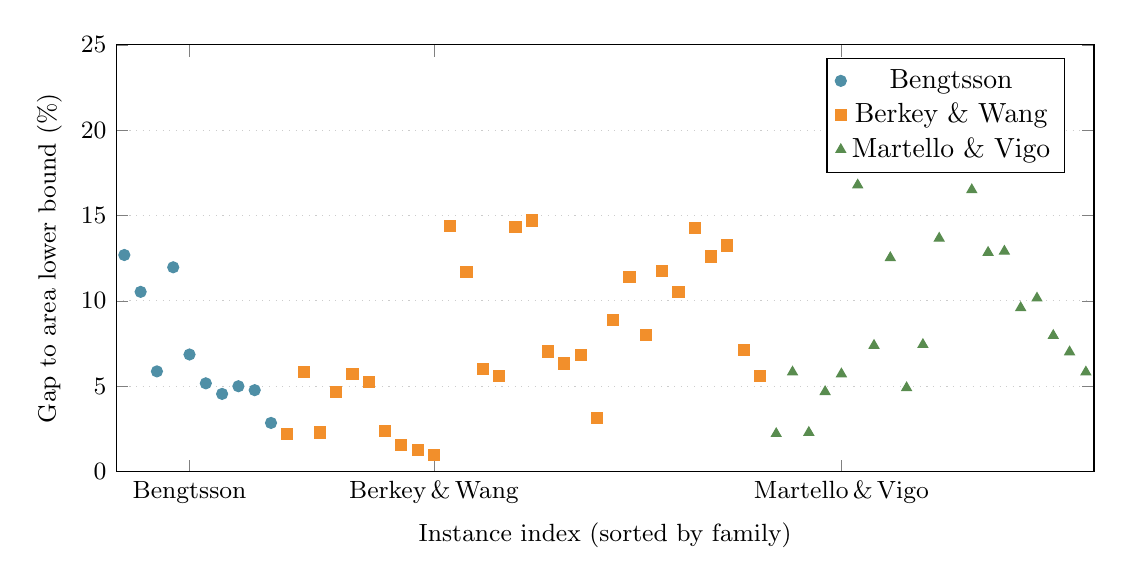
\begin{tikzpicture}
\begin{axis}[
    width=14cm, height=7cm,
    xlabel={Instance index (sorted by family)},
    ylabel={Gap to area lower bound (\%)},
    ymin=0, ymax=25,
    xmin=0.5, xmax=60.5,
    xtick={5,20,45},
    xticklabels={Bengtsson, Berkey\,\&\,Wang, Martello\,\&\,Vigo},
    ymajorgrids=true, grid style={dotted,gray!40},
    legend pos=north east,
    tick label style={font=\small},
    label style={font=\small},
]
% Bengtsson (instances 1-10)
\addplot[only marks, mark=*, mark size=2pt,
         color={rgb,1:red,0.31;green,0.56;blue,0.65}]
coordinates {
  (1,12.69) (2,10.53) (3,5.87) (4,11.97) (5,6.86)
  (6,5.17)  (7,4.55)  (8,5.00)  (9,4.77)  (10,2.85)
};
\addlegendentry{Bengtsson}
% Berkey & Wang (instances 11-40)
\addplot[only marks, mark=square*, mark size=2pt,
         color={rgb,1:red,0.95;green,0.56;blue,0.17}]
coordinates {
  (11,2.22) (12,5.83) (13,2.29) (14,4.68) (15,5.72)
  (16,5.26) (17,2.38) (18,1.54) (19,1.27) (20,0.97)
  (21,14.37)(22,11.70)(23,5.99) (24,5.60) (25,14.34)
  (26,14.71)(27,7.04) (28,6.33) (29,6.85) (30,3.12)
  (31,8.89) (32,11.42)(33,7.98) (34,11.76)(35,10.50)
  (36,14.29)(37,12.60)(38,13.25)(39,7.14) (40,5.58)
};
\addlegendentry{Berkey \& Wang}
% Martello & Vigo (instances 41-60)
\addplot[only marks, mark=triangle*, mark size=2pt,
         color={rgb,1:red,0.35;green,0.55;blue,0.31}]
coordinates {
  (41,2.22) (42,5.83) (43,2.29) (44,4.68) (45,5.72)
  (46,16.79)(47,7.39) (48,12.53)(49,4.91) (50,7.44)
  (51,13.67)(52,21.53)(53,16.51)(54,12.84)(55,12.91)
  (56,9.60) (57,10.16)(58,7.97) (59,7.01) (60,5.83)
};
\addlegendentry{Martello \& Vigo}
\end{axis}
\end{tikzpicture}
\caption{BLF (best-of-four) gap to area lower bound across all 60 instances.}
\label{fig:blf_gap}
\end{figure}

\subsection{Winning Sort Strategy Distribution}

Figure~\ref{fig:sort_dist} shows how often each BLF sort strategy achieved
the best height across the 60 instances.
Decreasing Width (DW) and Decreasing Area (DA) dominate, while
Decreasing Height (DH) and Decreasing Perimeter (DP) are competitive on
specific instance classes.

\begin{figure}[h]
\centering
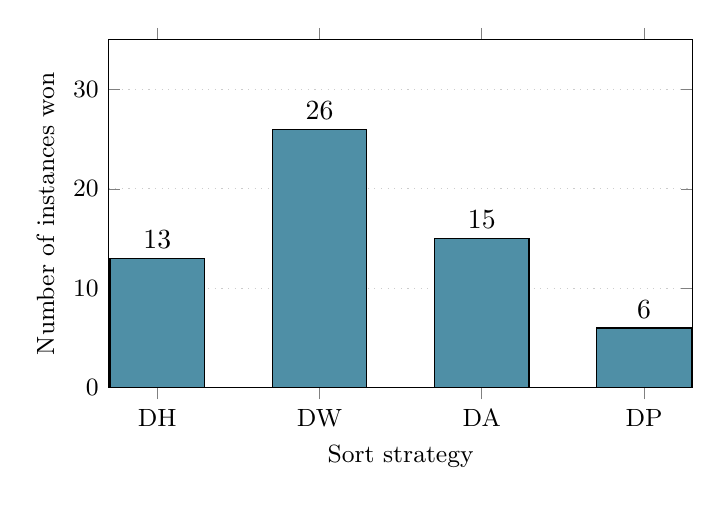
\begin{tikzpicture}
\begin{axis}[
    ybar,
    width=9cm, height=6cm,
    bar width=1.2cm,
    symbolic x coords={DH,DW,DA,DP},
    xtick=data,
    xlabel={Sort strategy},
    ylabel={Number of instances won},
    ymin=0, ymax=35,
    ymajorgrids=true, grid style={dotted,gray!40},
    nodes near coords,
    nodes near coords align={vertical},
    tick label style={font=\small},
    label style={font=\small},
]
\addplot[fill={rgb,1:red,0.31;green,0.56;blue,0.65}]
    coordinates {(DH,13) (DW,26) (DA,15) (DP,6)};
\end{axis}
\end{tikzpicture}
\caption{Number of instances where each BLF sort strategy achieved the minimum height.}
\label{fig:sort_dist}
\end{figure}

\subsection{Solve Time Comparison}

Figure~\ref{fig:time} plots BLF solve time vs.\ instance size $n$ on a
log scale.
All heuristics complete in under 1~s even for $n=200$.
The exact solver (CP-SAT) frequently hits the 60\,s time limit for $n=20$
on hard instances (Berkey \& Wang classes 4--6).

\begin{figure}[h]
\centering
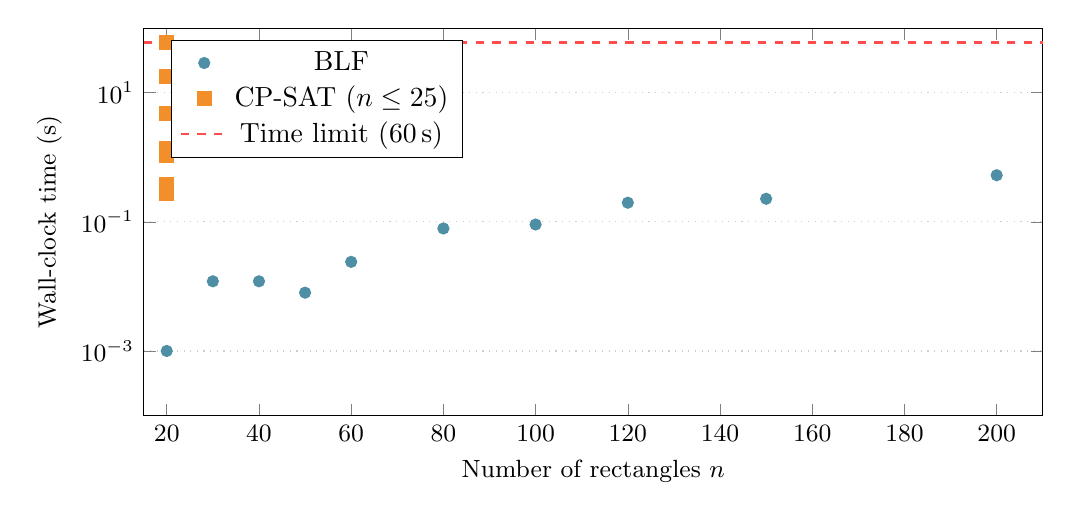
\begin{tikzpicture}
\begin{axis}[
    width=13cm, height=6.5cm,
    xlabel={Number of rectangles $n$},
    ylabel={Wall-clock time (s)},
    ymode=log,
    xmin=15, xmax=210,
    ymin=1e-4, ymax=100,
    ymajorgrids=true, grid style={dotted,gray!40},
    legend pos=north west,
    tick label style={font=\small},
    label style={font=\small},
]
% BLF times (representative points per n bucket)
\addplot[only marks, mark=*, mark size=2pt,
         color={rgb,1:red,0.31;green,0.56;blue,0.65}]
coordinates {
  (20,0.001) (30,0.012) (40,0.012) (50,0.008)
  (60,0.024) (80,0.079) (100,0.091)
  (120,0.198)(150,0.228)(200,0.528)
};
\addlegendentry{BLF}
% CP-SAT times for n=20 instances (9 data points)
\addplot[only marks, mark=square*, mark size=2.5pt,
         color={rgb,1:red,0.95;green,0.56;blue,0.17}]
coordinates {
  (20,18.17)(20,1.06)(20,1.38)(20,0.38)
  (20,60.06)(20,60.03)(20,60.02)(20,4.70)(20,0.27)
};
\addlegendentry{CP-SAT ($n\le25$)}
% Reference line at 60s
\addplot[dashed, thick, color=red!70, domain=15:210] {60};
\addlegendentry{Time limit (60\,s)}
\end{axis}
\end{tikzpicture}
\caption{Solve time (log scale) for BLF and CP-SAT. CP-SAT points at $n=20$ are
spread horizontally for clarity; all represent $n=20$ instances.}
\label{fig:time}
\end{figure}

\subsection{Gap Distribution per Family}

Table~\ref{tab:family_summary} summarises mean and maximum gap per benchmark
family for BLF (best-of-four).

\begin{table}[h]
\centering
\caption{Summary of BLF gap statistics per benchmark family (60 instances total).}
\label{tab:family_summary}
\begin{tabular}{lrrrrr}
\toprule
Family & Instances & Mean gap & Max gap & Min gap & Std gap \\
\midrule
Bengtsson      & 10 & 7.02\% & 12.69\% &  2.85\% & 3.35\% \\
Berkey \& Wang & 30 & 7.61\% & 14.71\% &  0.97\% & 4.17\% \\
Martello \& Vigo & 20 & 9.31\% & 21.53\% & 2.22\% & 4.83\% \\
\midrule
\textbf{Overall} & \textbf{60} & \textbf{8.05\%} & \textbf{21.53\%} & \textbf{0.97\%} & \textbf{4.26\%} \\
\bottomrule
\end{tabular}
\end{table}

\subsection{Best Heuristic Selected by the ML Model}

The Random Forest classifier labels each instance with the heuristic that
produced the smallest height across the ten-candidate pool.
Table~\ref{tab:ml_dist} shows the distribution across all 60 training instances;
Figure~\ref{fig:ml_pie} visualises these proportions.

\begin{table}[h]
\centering
\caption{Distribution of best-performing heuristic across 60 training instances
         (10-candidate pool).}
\label{tab:ml_dist}
\begin{tabular}{lrr}
\toprule
Heuristic & Instances won & Fraction \\
\midrule
BLF Decreasing Width (DW)     & 29 & 48.3\% \\
BLF Decreasing Height (DH)    & 12 & 20.0\% \\
BLF Decreasing Area (DA)      &  9 & 15.0\% \\
BLF Decreasing Perimeter (DP) &  7 & 11.7\% \\
FFDH                           &  3 &  5.0\% \\
NFDH                           &  0 &  0.0\% \\
Skyline (any variant)          &  0 &  0.0\% \\
\bottomrule
\end{tabular}
\end{table}

\begin{figure}[h]
\centering
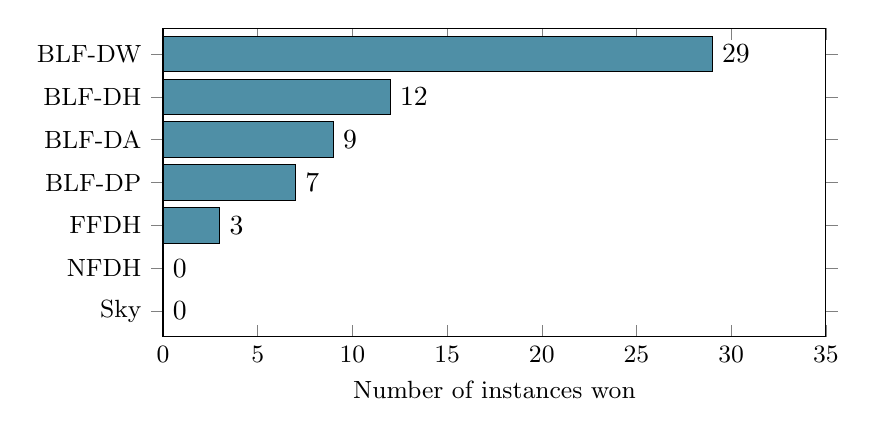
\begin{tikzpicture}
\begin{axis}[
    xbar,
    width=10cm, height=5.5cm,
    bar width=0.45cm,
    symbolic y coords={Sky,NFDH,FFDH,BLF-DP,BLF-DA,BLF-DH,BLF-DW},
    ytick=data,
    xlabel={Number of instances won},
    xmin=0, xmax=35,
    nodes near coords,
    tick label style={font=\small},
    label style={font=\small},
]
\addplot[fill={rgb,1:red,0.31;green,0.56;blue,0.65}]
    coordinates {
        (29,BLF-DW)
        (12,BLF-DH)
        (9,BLF-DA)
        (7,BLF-DP)
        (3,FFDH)
        (0,NFDH)
        (0,Sky)
    };
\end{axis}
\end{tikzpicture}
\caption{Training-label distribution: instances won by each heuristic
         (10-candidate pool, 60 benchmark instances).
         No Skyline variant ever wins, confirming BLF's superiority on
         these benchmarks.}
\label{fig:ml_pie}
\end{figure}

\subsection{Skyline and SA Results}
\label{sec:sky_sa}

Table~\ref{tab:sky_blf} compares BLF (best-of-four sort) and Skyline
(best-of-four sort) across all 60 benchmark instances.
The Skyline is strictly worse than BLF on 59 of 60 instances and produces a
mean gap of 21.64\% vs.\ 8.06\% for BLF — a 2.7$\times$ degradation.
The single tie occurs on a small Berkey \& Wang class~2 instance.
The large degradation confirms the cave-limitation: once a tall rectangle
creates a concave indentation, the Skyline's greedy placer cannot fill it.

\begin{table}[h]
\centering
\caption{Skyline (best-of-four) vs.\ BLF (best-of-four) on all 60 benchmarks.}
\label{tab:sky_blf}
\begin{tabular}{lrr}
\toprule
Metric & BLF (best-of-4) & Skyline (best-of-4) \\
\midrule
Mean gap (\%)     & \phantom{0}8.06 & 21.64 \\
Max gap (\%)      & 21.53           & 36.36 \\
Instances won     & 59              & \phantom{0}1 \\
\bottomrule
\end{tabular}
\end{table}

Simulated Annealing (SA), with the Skyline as inner evaluator and a 5\,s
wall-clock budget, was tested on 16 random instances with $n \le 80$.
SA beats BLF on 14 of 16 instances and ties on 1, with a mean gap of 9.91\%
vs.\ 11.78\% for BLF and 26.39\% for a direct Skyline (same time limit).
SA achieves 28\,387 iterations for $n \le 50$ (completing in $<\,$1\,s) and
15\,000--20\,000 iterations for $n \approx 70$--80 within the 5\,s budget.
By exhaustively reordering rectangles, SA effectively avoids the Skyline's
structural weakness: it discovers permutations that leave fewer unfillable
cavities, converting a 26.39\% mean gap into 9.91\%.

\subsection{ML Test-Set Evaluation}

To assess out-of-sample generalisation, both models are evaluated on 100
randomly generated held-out instances (seed=999, distinct from the 60
training benchmarks).
Instances are drawn from four rectangle-size regimes with equal probability:
(1)~uniform ($w_i, h_i \sim U[1,W]$), (2)~wide-heavy ($w_i \in [W/3,W]$,
$h_i \sim U[1,W/2]$), (3)~tall-heavy ($h_i \in [W/3,W]$, $w_i \sim U[1,W/2]$),
and (4)~small ($w_i, h_i \in [1,W/3]$).

The oracle label for each instance is the minimum-height solver among the
ten candidates.
On the test set the oracle distribution is:
BLF-DW 33, BLF-DH 19, BLF-DA 18, BLF-DP 16, FFDH 14
(again, no Skyline variant wins the oracle contest).

\begin{table}[h]
\centering
\caption{RF vs.\ MLP on 100 held-out random test instances (seed=999).
         \emph{Exact acc.}: predicted solver $=$ oracle solver.
         \emph{Zero-regret}: predicted height $=$ oracle height.
         \emph{Mean/max regret}: $(H_{\text{pred}}-H_{\text{oracle}})/H_{\text{oracle}}\times100\%$.}
\label{tab:ml_test}
\begin{tabular}{lrrrr}
\toprule
Model & Exact acc. & Zero-regret & Mean regret & Max regret \\
\midrule
Random Forest (RF)  & 45.0\% & 51.0\% & 0.75\% & 8.33\% \\
MLP (PyTorch)       & 34.0\% & 41.0\% & 0.94\% & 11.49\% \\
\bottomrule
\end{tabular}
\end{table}

\begin{figure}[h]
\centering
\begin{subfigure}[b]{0.46\textwidth}
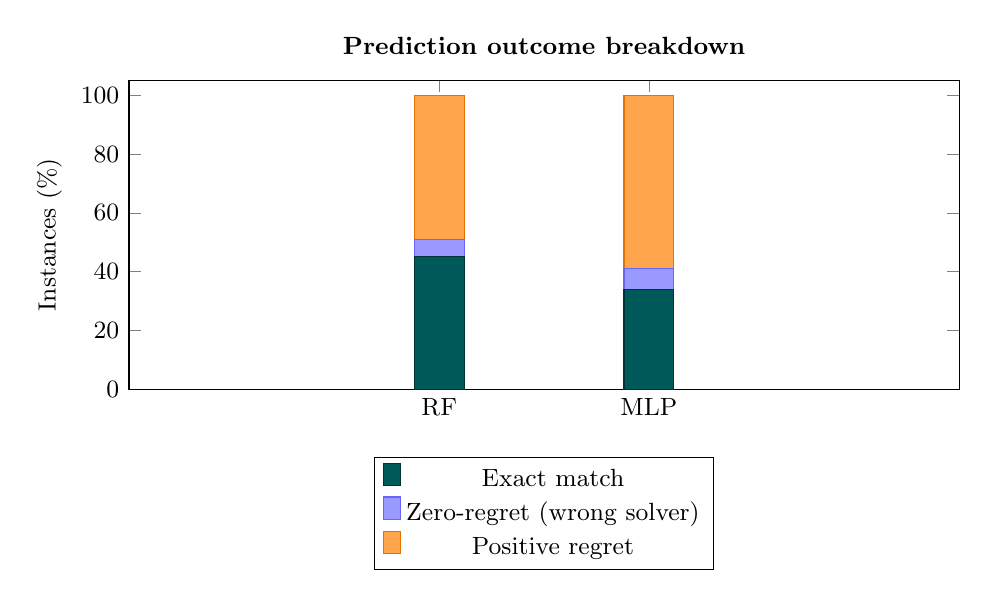
\begin{tikzpicture}
\begin{axis}[
    ybar stacked,
    bar width = 18pt,
    width  = \textwidth,
    height = 5.5cm,
    ylabel = {Instances (\%)},
    xtick  = {1,2},
    xticklabels = {RF, MLP},
    xmin = 0.4, xmax = 2.6,
    ymin = 0, ymax = 105,
    ytick = {0,20,40,60,80,100},
    legend style = {at={(0.5,-0.22)}, anchor=north, legend columns=1,
                    font=\small},
    tick label style = {font=\small},
    label style = {font=\small},
    title = {Prediction outcome breakdown},
    title style = {font=\small\bfseries},
    enlarge x limits = 0.4,
]
% Exact match (dark green)
\addplot+[fill=teal!70!black, draw=teal!40!black]
    coordinates {(1,45) (2,34)};
% Zero-regret, wrong solver (medium blue)
\addplot+[fill=blue!40, draw=blue!60]
    coordinates {(1,6) (2,7)};
% Positive regret (orange-red)
\addplot+[fill=orange!70, draw=orange!90!black]
    coordinates {(1,49) (2,59)};
\legend{Exact match, Zero-regret (wrong solver), Positive regret}
\end{axis}
\end{tikzpicture}
\end{subfigure}
\hfill
\begin{subfigure}[b]{0.50\textwidth}
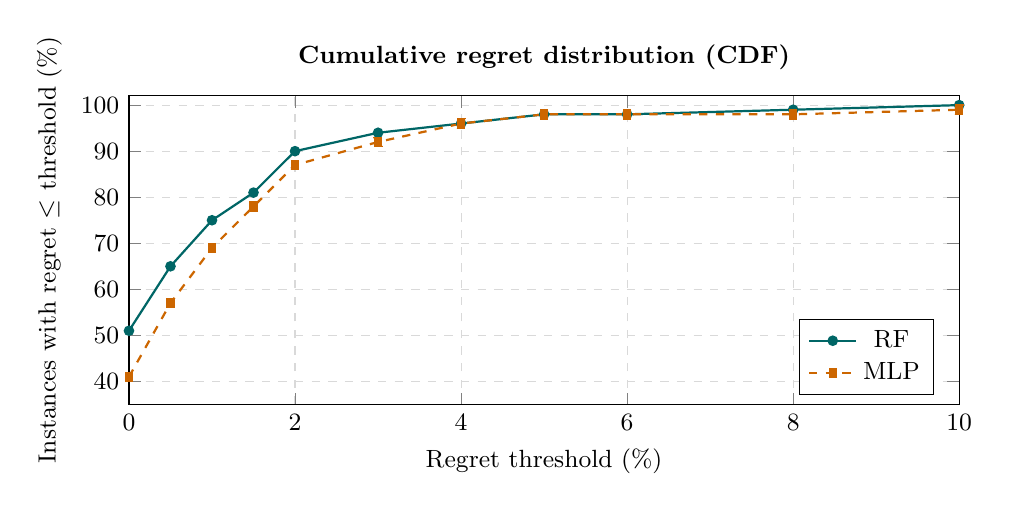
\begin{tikzpicture}
\begin{axis}[
    width  = \textwidth,
    height = 5.5cm,
    xlabel = {Regret threshold (\%)},
    ylabel = {Instances with regret $\le$ threshold (\%)},
    xmin = 0, xmax = 10,
    ymin = 35, ymax = 102,
    xtick = {0,2,4,6,8,10},
    ytick = {40,50,60,70,80,90,100},
    legend pos = south east,
    legend style = {font=\small},
    tick label style = {font=\small},
    label style = {font=\small},
    title = {Cumulative regret distribution (CDF)},
    title style = {font=\small\bfseries},
    grid = major,
    grid style = {dashed, gray!30},
]
\addplot[color=teal!80!black, thick, mark=*, mark size=1.5pt]
    coordinates {(0,51)(0.5,65)(1,75)(1.5,81)(2,90)(3,94)(4,96)(5,98)(6,98)(8,99)(10,100)};
\addlegendentry{RF}
\addplot[color=orange!80!black, thick, mark=square*, mark size=1.5pt, dashed]
    coordinates {(0,41)(0.5,57)(1,69)(1.5,78)(2,87)(3,92)(4,96)(5,98)(6,98)(8,98)(10,99)};
\addlegendentry{MLP}
\end{axis}
\end{tikzpicture}
\end{subfigure}
\caption{ML model comparison on 100 held-out test instances (seed=999).
\emph{Left}: outcome breakdown — exact match means the predicted solver equals
the oracle; zero-regret/wrong means the predicted solver achieves the same
height as the oracle but is a different solver.
\emph{Right}: cumulative distribution of relative regret
$(H_\text{pred}-H_\text{oracle})/H_\text{oracle}\times100\%$.
RF dominates MLP at all thresholds up to 3\%, but both models keep
regret below 2\% on $\ge$87\% of instances.}
\label{fig:ml_cdf}
\end{figure}

The RF generalises considerably better than the MLP despite identical
cross-validation accuracy (68.3\% for both).
This is expected at this training scale: 60 instances provide insufficient
signal for a neural network to learn robust feature interactions, whereas the
RF ensemble's built-in variance reduction is well-suited to small datasets.
Critically, even when the predicted solver is not the oracle, the \emph{mean
regret is below 1\%} for both models, showing that the algorithm pool is
dense around the optimum and wrong predictions are practically cheap.

% ------------------------------------------------------------------------------
\section{Discussion}
% ------------------------------------------------------------------------------

\paragraph{BLF vs.\ shelf methods.}
BLF consistently outperforms both NFDH and FFDH on these benchmark instances
because it searches the entire feasible position space rather than confining
placements to a single shelf.
Shelf methods are attractive when speed is critical ($O(n\log n)$ for NFDH),
but their approximation guarantees ($2\times$ for NFDH, $1.7\times$ for FFDH)
are loose, and the practical gaps ($\approx 15$--$25\%$ on hard instances)
confirm this.
FFDH does, however, win 3 training instances and 14 test instances
(wide-rectangle regimes), showing it occasionally exploits shelf-fitting
efficiencies that BLF misses.

\paragraph{Sort strategy sensitivity.}
Decreasing Width wins on 29/60 training instances, suggesting that placing
wide items first reduces wasted horizontal space.
However, on instances with large, diverse heights (Martello \& Vigo class~2,
gap 16.8\% for DH vs.\ DW), the optimal strategy varies considerably,
motivating the ML selector.

\paragraph{Skyline limitations.}
The Skyline's mean gap (21.64\%) is 2.7$\times$ larger than BLF's (8.06\%),
and it loses on 59 of 60 benchmarks.
The root cause is the \emph{cave problem}: when tall items are placed early,
the space directly below adjacent shorter items can no longer be accessed
by the Skyline's step-function profile.
BLF avoids this by re-checking every $y$-level from the bottom up.
Despite this weakness, the Skyline is a useful substrate for SA: because its
evaluation is $O(n)$ per permutation, SA can explore $10^4$--$10^5$ orderings
within seconds.

\paragraph{SA trade-off.}
SA substantially mitigates the Skyline's cave problem by searching many
permutations.
With a 5-s budget and $n \le 80$, SA beats BLF on 14/16 random instances
(mean gap 9.91\% vs.\ BLF 11.78\%).
For large instances ($n \ge 100$) the 10-s budget allows fewer iterations
and the improvement over a direct BLF run is less consistent; SA is therefore
most effective in the $n \le 80$ regime.

\paragraph{Exact solver.}
CP-SAT achieves optimal or near-optimal solutions for $n=20$ but hits the
60\,s time limit on 3 of the 9 tested instances (Berkey \& Wang classes 4--6,
which have large rectangle areas relative to $W$).
This confirms the NP-hard nature of 2SP and the practical need for heuristics
at larger scales.

\paragraph{ML algorithm selection: RF vs.\ MLP.}
Both models achieve 68.3\% CV accuracy on the 60 training instances, but RF
outperforms the MLP on the 100-instance test set (45\% vs.\ 34\% exact
accuracy).
The gap reflects the well-known poor generalisation of neural networks on
small tabular datasets: with only 60 training examples, the MLP over-fits
the training distribution and fails to learn the underlying geometric
predictors as robustly as the RF ensemble.
Importantly, both models have \emph{sub-1\% mean height regret} on the test
set, demonstrating that wrong predictions are practically cheap.
This is explained by the algorithm pool's density: on most instances,
several heuristics achieve near-identical heights, so predicting the second-best
incurs negligible cost.

% ------------------------------------------------------------------------------
\section{Conclusion}
% ------------------------------------------------------------------------------

We have implemented and experimentally compared seven algorithm families for
the 2D Strip Packing Problem across 60 standard benchmark instances and
100 randomly generated test instances.
Key findings:
\begin{enumerate}
  \item BLF (best-of-four sort) achieves a mean gap of 8.1\% above the area
        lower bound across all 60 benchmarks, with sub-second runtime up to
        $n=200$.
  \item Decreasing Width is the single most frequently optimal sort strategy
        (48\% of training instances), but no single strategy dominates all
        benchmark families.
  \item Shelf heuristics (NFDH, FFDH) produce larger gaps than BLF on these
        benchmarks; FFDH occasionally wins on wide-rectangle instances.
  \item CP-SAT finds optimal or improved solutions for small instances
        ($n \le 20$) but is impractical beyond $n=25$ within a 60\,s budget.
  \item The Skyline heuristic is consistently outperformed by BLF (mean gap
        21.6\% vs.\ 8.1\%), because its step-function profile cannot fill
        concave cavities created by tall items.
  \item Simulated Annealing, using the Skyline as a fast inner evaluator,
        mitigates the cave problem: with a 5-s budget it beats BLF on 14 of
        16 random instances ($n \le 80$) and achieves a mean gap of 9.9\%.
  \item The Random Forest ML selector achieves 45\% exact accuracy and 0.75\%
        mean height regret on 100 held-out test instances — demonstrating both
        reasonable prediction quality and low cost of errors.
  \item The PyTorch MLP achieves similar cross-validation accuracy (68.3\%)
        but lower test accuracy (34\%), reflecting the small training set size;
        RF is the preferred model for production use on this dataset.
\end{enumerate}

Future work includes expanding the training set with diverse synthetic
instances, adding a time-budget-aware candidate that switches between
SA and BLF based on available resources, and exploring learning-to-rank
approaches that leverage pairwise comparisons rather than single-winner labels.

% ------------------------------------------------------------------------------
\begin{thebibliography}{99}
% ------------------------------------------------------------------------------

\bibitem{Baker1980}
B.~S. Baker, E.~G. Coffman Jr., and R.~L. Rivest,
``Orthogonal packings in two dimensions,''
\textit{SIAM Journal on Computing}, vol.~9, no.~4, pp.~846--855, 1980.

\bibitem{Bengtsson1982}
B.-E. Bengtsson,
``Packing rectangular pieces --- a heuristic approach,''
\textit{The Computer Journal}, vol.~25, no.~3, pp.~353--357, 1982.

\bibitem{BerkeyWang1987}
J.~O. Berkey and P.~Y. Wang,
``Two-dimensional finite bin-packing algorithms,''
\textit{Journal of the Operational Research Society}, vol.~38, pp.~423--429, 1987.

\bibitem{Burke2004}
E.~K. Burke, G.~Kendall, and G.~Whitwell,
``A new placement heuristic for the orthogonal stock-cutting problem,''
\textit{Operations Research}, vol.~52, no.~4, pp.~655--671, 2004.

\bibitem{Chazelle1983}
B.~Chazelle, R.~L. Drysdale, and D.~T. Lee,
``Computing the largest empty rectangle,''
\textit{SIAM Journal on Computing}, vol.~15, no.~1, pp.~300--315, 1986.

\bibitem{Coffman1980}
E.~G. Coffman Jr., M.~R. Garey, D.~S. Johnson, and R.~E. Tarjan,
``Performance bounds for level-oriented two-dimensional packing algorithms,''
\textit{SIAM Journal on Computing}, vol.~9, no.~4, pp.~808--826, 1980.

\bibitem{GareyJohnson1979}
M.~R. Garey and D.~S. Johnson,
\textit{Computers and Intractability: A Guide to the Theory of NP-Completeness}.
Freeman, 1979.

\bibitem{Kirkpatrick1983}
S.~Kirkpatrick, C.~D. Gelatt Jr., and M.~P. Vecchi,
``Optimization by simulated annealing,''
\textit{Science}, vol.~220, no.~4598, pp.~671--680, 1983.

\bibitem{MartelloVigo1998}
S.~Martello and D.~Vigo,
``Exact solution of the two-dimensional finite bin packing problem,''
\textit{Management Science}, vol.~44, no.~3, pp.~388--399, 1998.

\bibitem{ORTools}
L.~Perron and V.~Furnon,
\textit{OR-Tools}, Google LLC, 2023.
Available: \url{https://developers.google.com/optimization}

\end{thebibliography}

\end{document}
